
\begin{figure*}[t]
	\centering
	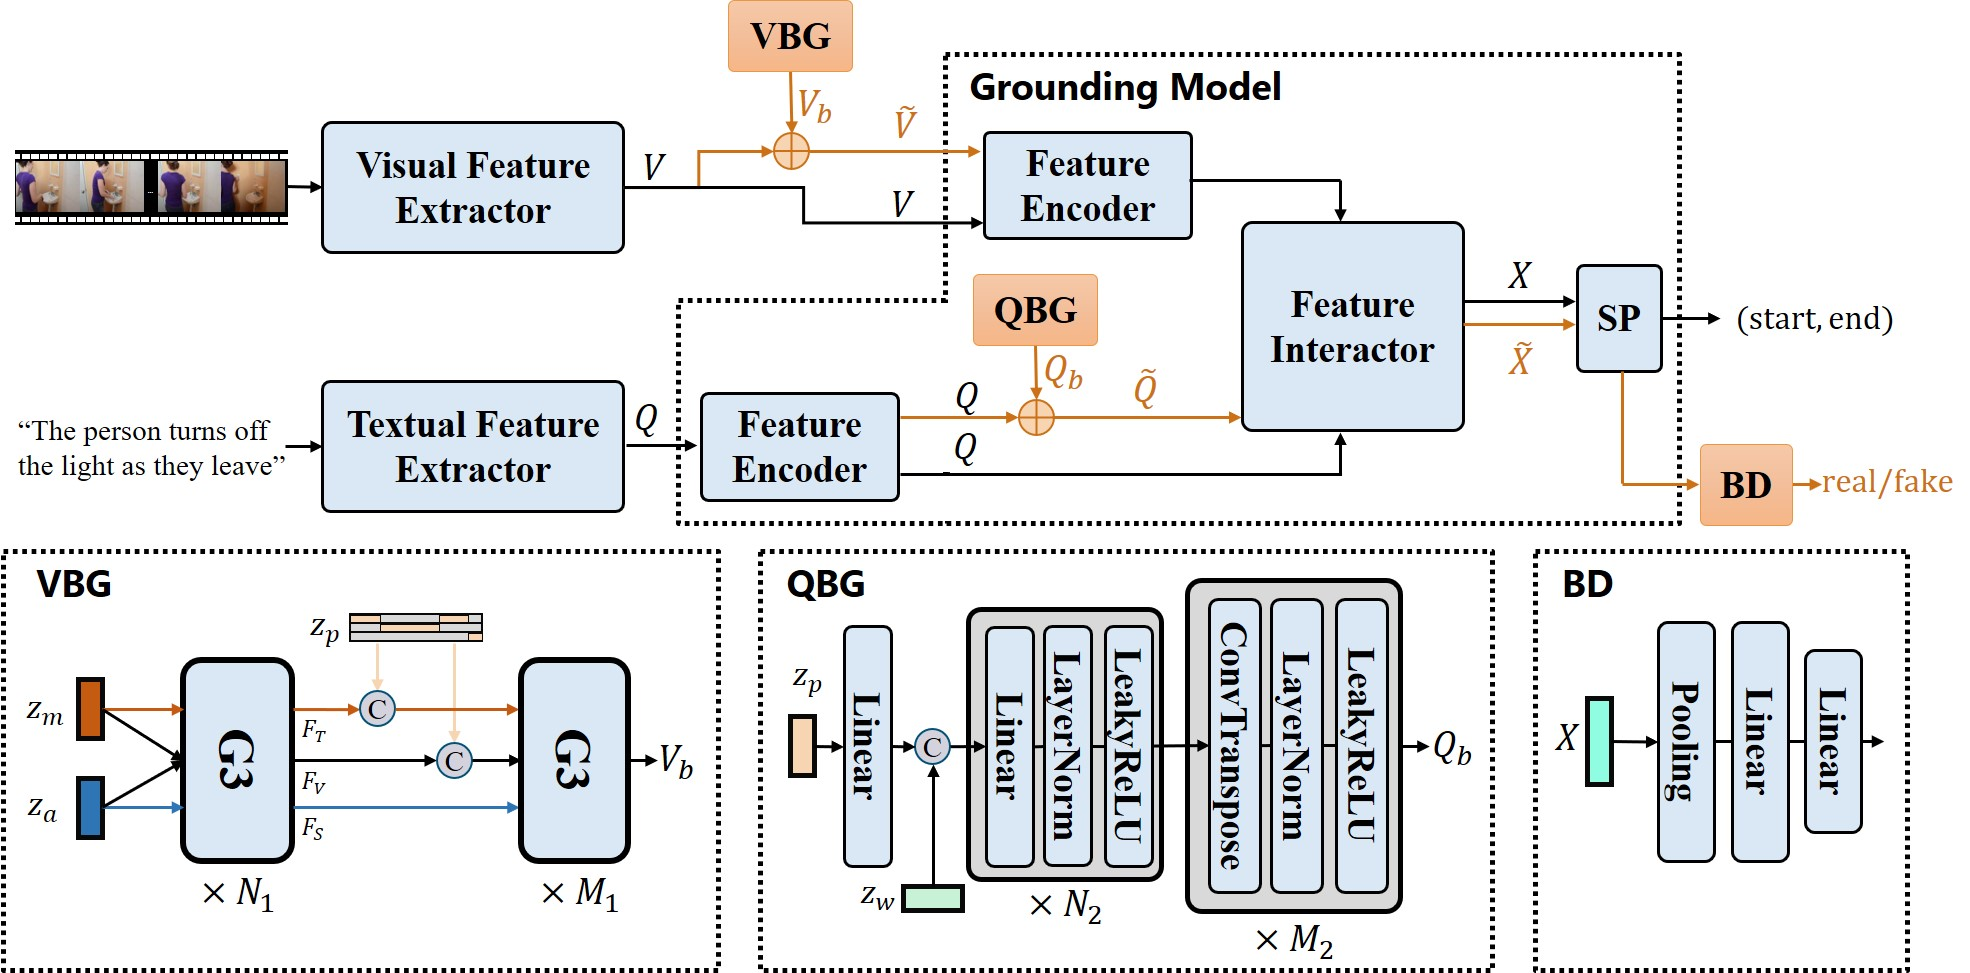
\includegraphics[width=0.96\linewidth]{images/OverView.jpg}%-crop.pdf}
	\caption{An overview of our BSSARD. The orange background is only used during the training period. Best viewed in color.}
	%\vspace{-3mm}
	\label{Overview}
\end{figure*}


\section{Method}


\subsection{Overview}

Our bias-conflict sample synthesis and adversarial removal debias strategy (BSSARD) is shown in Figure~\ref{Overview}, which is based on a span-based grounding model and incorporates a Visual Bias Generator (VBG), a Query Bias Generator (QBG), and a Bias Discriminator (BD). 

In the training stage, given a video-query pair~$(I_v,I_q)$ with the target moment~$(y_s^r,y_e^r)$ , we first utilize the visual and textual feature extractor to capture feature representations $V$ and $Q$. 
On the one hand, we feed the original $V$ and $Q$ into the feature encoder and feature interactor to obtain real sample feature $X$. Then, the span predictor (SP) should accurately produce the start and end time of the target moment. Meanwhile, the bias discriminator module should accurately predict it as the real sample. 
On the other hand, given a fake temporal location $z_p=(y_s^f, y_e^f)$ of the target moment obtained through random uniform sampling from the video frames, we employ VBG to generate visual bias feature $V_b$ and element-wise add it to the real sample feature $V$, which produces $\tilde{V}$. Similar to the real sample, we obtain bias-conflict sample feature $\tilde{X}$. It has two labels, one is the temporal position $(y_s^r,y_e^r)$ of the real target moment and the other is the fake temporal position $(y_s^f, y_e^f)$. The bias generator wants to generate shortcut features to trick SP into generating a target moment similar to $z_p$ and trick BD into judging the current sample as the real sample. Instead, the SP will try to generate target moments as close as $(y_s^r,y_e^r)$ and the BD will judge it as a sample with bias. 
Similarly, we also employ QBG to generate textual bias feature $Q_b$ and perform the above process. 
The synthesized bias features simulate all kinds of spurious correlations between the semantic information of video/text and the temporal position of the target clips. Through adversarial training, it effectively mitigates visual and linguistic biases. 
In the inference stage, the VBG, QBG, and BD components are removed. 


\subsection{Bias Generator}
% We implement a visual bias generator and a query bias generator to model visual bias and language bias respectively. 
%is a conditional generator that 

The bias generator generates bias-conflict sample features based on synthesized spurious relationships between the unimodality information and the temporal positional labels. 


\subsubsection{Visual Bias Generator} 

We construct VBG by the $\text{G}^\text{3}$ module~\cite{G3AN}, which encodes video features by decoupling appearance and motion content. The VBG contains three randomly generated variables $z_a$, $z_m$, and $z_p$ as inputs, and generates visual bias vector $V_{b}$ for constructing bias-conflict samples. These random variables guarantee the diversity and randomness of the bias generator.

Especially, the $z_a$ and $z_m$ are random vectors that follow a normal distribution and represent appearance and motion content, respectively. 
VBG first inputs $z_a$ and $z_m$ into $N_1$ stacked $\text{G}^\text{3}$, and produces three visual stream features, named temporal stream $F_T$, spatial stream $F_S$ and video stream $F_V$. 
Then, we random generate a fake temporal label $z_p \in \mathbb{R}^{3 \times n}$ of the target clip, which is obtained through random uniform sampling from the video frame sequence within the range of $\left[0, n-1\right]$. Its three dimensions are mutually exclusive and represent whether the segment contains background, foreground, or ignored data. It provides the temporal position conditional information that the bias generator requires. Subsequently, $z_p$ is concatenated with $F_T$ and $F_V$ to introduce temporal position information. 
Next, VBG outputs the visual bias vector $V_b\in \mathbb{R}^{n \times d}$ through $M_1$ stacked $\text{G}^\text{3}$. Finally, we add $V_b$ to $V$ and obtain visual bias conflict sample feature $\tilde{V}$,
\begin{equation}
	\begin{split}
		V_{b} &= VBG\left(z_a, z_m, z_p\right)\\
		\tilde{V} &= V_b + V
	\end{split}	
	\label{eq1}
\end{equation}
where $n$ and $d$ are the video length and feature dimension.


\subsubsection{Query Bias Generator}

We construct QBG by a simple fully connected structure and transpose convolutional structure. 
The QBG needs two randomly generated variables $z_w$ and $z_p$ as inputs and generates textual bias vector $Q_{b}$ for constructing bias-conflict samples. 

Specifically, we randomly sample $z_p$ from a normal distribution, which is a random vector of length $n$ and represents the synthetic label of the fake target video moment. Then we embed it using a fully connected layer, which provides the temporal position information for the feature generation. 
To enhance randomness and diversity, QBG also generates a random vector $z_w$ from a normal distribution to introduce the context for the feature generation, which is concatenated with the encoded position feature. 
We use $N_2$ linear layers and $M_2$ transposed convolution layers to produce the word sequence bias feature $Q_b\in \mathbb{R}^{m \times d}$. Finally, we add $Q_b$ to $Q$ and obtain query bias conflict sample feature $\tilde{Q}$,
\begin{equation}
	\begin{split}
		Q_b &= QBG\left(z_w, z_p\right)\\ 
		\tilde{Q} &= Q_b + Q
	\end{split}
	\label{eq2}
\end{equation}
where $m$ represents the length of the query text.


\subsection{Grounding Model}

The grounding model consists of a feature encoder, feature interactor, span predictor (SP), and bias discriminator (BD). 
BD is a binary classifier that identifies whether the sample contains biases. 
SP should make correct temporal grounding predictions for both regular and bias-conflict samples. 

For the normal samples without synthetic bias features, $V$ and $Q$ are encoded by the feature encoder and feature interactors to generate cross-modal representations $X$. Subsequently, the SP and BD make predictions, 
\begin{equation}
	\begin{split}
		p_{s}^r, p_{e}^r &= SP(X) \in \mathbb{R}^{n}, \mathbb{R}^{n}\\
		p_{d}^r &= BD(X) \in \mathbb{R}^{2}
	\end{split}
	\label{eq3}
\end{equation}
where $p_{s}^r$ and $p_{e}^r$ represent the predicted start and end positions of the target moment for the real sample, and $p_{d}^r$ represents the probability of the sample containing bias.

For bias-conflict samples, we iteratively encode $\tilde{V}$ and $Q$ or $V$ and $\tilde{Q}$ in each training iteration by the feature encoder and feature interactor to generate cross-modal representation $\tilde{X}$. Subsequently, the SP and BD make predictions,
\begin{equation}
	\begin{split}
		p_{s}^f, p_{e}^f &= SP(\tilde{X}) \in \mathbb{R}^{n}, \mathbb{R}^{n}\\
		p_{d}^f &= BD(\tilde{X}) \in \mathbb{R}^{2}
	\end{split}
	\label{eq4}
\end{equation}
where $p_{s}^f$ and $p_{e}^f$ represent the predicted start and end positions of the target moment for the bias-conflict sample, and $p_{d}^f$ represents the probability of the sample containing bias.


\subsection{Training Objectives}

\subsubsection{Training Process}

As shown in Algorithm~\ref{Training Process}, we train the two bias generators alternately in each training step. We detail the bias generator loss $L^g$ and the discriminator loss $L^d$.


\begin{algorithm}[t]
	\caption{Training process in one epoch.}
	\label{Training Process}
	\begin{algorithmic}[1] %这个1 表示每一行都显示数字
		\REQUIRE $\text{VBG}$; $\text{QBG}$; $\text{GD}$;
		\ENSURE TSGV model
		\FOR{each training iteration}
		\STATE Sample $\left(V, Q \right)$, $(y_s^r,y_e^r)$
		\STATE Sample $z_m$, $z_a$, $z_p$, $(y_s^f,y_e^f)$
		\STATE $V_b \leftarrow \text{VBG}(z_m, z_a, z_p)$
		\STATE $\tilde{V} \leftarrow V + V_b$, $\tilde{Q} \leftarrow Q$
		\STATE Get $p_{s}^r, p_{e}^r, p_{d}^r, p_{s}^f, p_{e}^f, p_{d}^f$ by Equation~\ref{eq3} and~\ref{eq4} 
		\STATE Calculate $L^g$ and train VBG, freeze GD
		\STATE Calculate $L^d$ and train GD, freeze VBG
		
		\STATE Sample $z_w$, $z_p$, $(y_s^f,y_e^f)$
		\STATE $Q_b \leftarrow \text{QBG}(z_w, z_p)$
		\STATE $\tilde{V} \leftarrow V$, $\tilde{Q} \leftarrow Q + Q_b$
		\STATE Get $p_{s}^r, p_{e}^r, p_{d}^r, p_{s}^f, p_{e}^f, p_{d}^f$ by Equation~\ref{eq3} and~\ref{eq4} 
		\STATE Calculate $L^g$ and train QBG, freeze GD
		\STATE Calculate $L^d$ and train GD, freeze QBG
		\ENDFOR
	\end{algorithmic}
\end{algorithm}


\subsubsection{Bias Generator Training Objectives}
The visual/query bias generator aims to deceive the bias discriminator and induce the span predictor to produce the given fake labels.

We use cross-entropy loss to trick the bias discriminator,
\begin{equation}
	L_{cls}^g=f_{CE}(p_{d}^f, 0)
	\label{g_loss_cls}
\end{equation}
where $p_d^f$ represents the predicted sample flag. $0$ indicates the current sample is a real sample without synthetic bias. It encourages the generator to generate samples that the BD will classify as unbiased. 

To induce span predictor, we use cross-entropy loss:
\begin{equation}
	L_{loc}^g=\frac{1}{2}\left[f_{CE}\left(p_{s}^{f}, y_{s}^{f}\right)+f_{CE}\left(p_{e}^{f}, y_{e}^{f}\right)\right]
	\label{g_loss_loc}
\end{equation}
This encourages the bias generator to generate bias-conflict samples that can deceive the grounding model.

The total training loss of the bias generator is
\begin{equation}
	L^{g}=L_{loc}^g+\lambda_{1} L_{cls}^g
	\label{g_loss}
\end{equation}
where $\lambda_{1}$ is a weight hyperparameter.


\subsubsection{Discriminator Training Objectives}
The discriminator needs to distinguish between real and bias-conflict samples and predict the true target moments.

For the bias discriminator, we use cross-entropy loss,
\begin{equation}
	L_{cls}^d=f_{CE}(p_{d}^r, 0) + f_{CE}(p_{d}^f, 1)
	\label{d_loss_cls}
\end{equation}
It encourages the discriminator to accurately judge real and synthetic samples.

For the temporal grounding, we use the traditional span-based cross-entropy loss,
\begin{equation}
	\begin{split}
		L_{loc}^d =&\frac{1}{2}\left[f_{CE}\left(p_{s}^{r}, y_{s}^{r}\right)+f_{CE}\left(p_{e}^{r}, y_{e}^{r}\right)\right]\\
		+& \frac{1}{2}\left[f_{CE}\left(p_{s}^{f}, y_{s}^{r}\right)+f_{CE}\left(p_{e}^{f}, y_{e}^{r}\right)\right]\\
	\end{split}
	\label{d_loss_loc}
\end{equation}

Besides, we find it advantageous to incorporate a sample-based distance metric such as KL divergence. Consequently, we introduce an additional objective, 
\begin{equation}
	L^d_{kl} = D_{kl}(p_{s}^{r} \| p_{s}^{f}) + D_{kl}(p_{e}^{r} \| p_{e}^{f})
	\label{loss_kl_d}
\end{equation}
Here, Equation~\ref{d_loss_loc} aligns the predictions towards the real labels, and Equation~\ref{loss_kl_d} limits the predictions of bias-conflict samples to not deviate much from the predictions of the corresponding original samples. 
Meanwhile, KL divergence is a regularization method to prevent the generator from overfitting training data and improve the generalization ability. 


\begin{table*}[t]
	\centering
	% \small
	\renewcommand{\arraystretch}{1}
	\setlength{\tabcolsep}{1.4mm}
	\begin{tabular}{c c c c | c c c|c c c | c c c}
		\toprule
		\multirow{3}{*}{Method}
		& \multicolumn{6}{c}{Charades-CD} & \multicolumn{6}{c}{ActivityNet-CD} \\
		& \multicolumn{3}{c}{OOD} & \multicolumn{3}{c}{IID} & \multicolumn{3}{c}{OOD} & \multicolumn{3}{c}{IID}\\
		& r1i5 & r1i7 & mIoU & r1i5 & r1i7 & mIoU & r1i5 & r1i7 & mIoU & r1i5 & r1i7 & mIoU \\
		\midrule
		2D-TAN~\cite{RN2} & 28.18 & 13.73 & 34.22 & 46.48 & 28.76 & 42.73 & 18.86 & 9.77 & 28.31 & 40.87 & 28.95 & 44.99\\
		
		LG~\cite{RN21} & 42.90 & 19.29 & 39.43 & 51.28 & 28.68 & 45.16 &
		23.85 & 10.96 & 28.46 & 46.41 & 29.28 & 44.62\\
		
		DRN~\cite{RN20} & 31.11 & 15.17 & 23.05 & 42.04 & 23.32 & 28.21 & 
		- & - & - & - & - & -\\
		
		VSLNet~\cite{RN4} & 34.10 & 17.87 & 36.34 & 43.26 & 28.43 & 42.92 &
		20.03 & 10.29 & 28.18 & 47.81 & 29.07 & 46.33\\
		
		DCM~\cite{RN29} & 40.51 & 21.02 & 40.99 & 52.50 & 35.28 & 48.74 & 20.86 & 11.07 & 28.08 & 42.15 & 29.69 & 45.20\\
		
		SVTG~\cite{RN30} & 46.67 & 27.08 & 44.30 & 57.59 & 37.79 & 50.93 &
		24.57 & 13.21 & 30.45 & 48.07 & 32.15 & 47.03\\
		
		MDD~\cite{lan2022closer} & 40.39 & 22.70 & - & 52.78 & 34.71 & - & 20.80 & 11.66 & - & 43.63 & 31.44 & - \\
		
		\midrule
		QAVE~\cite{hao2022query} & 37.84 & 19.67 & 38.45 & 47.63 & 29.28 & 44.17 &
		21.39 & 10.86 & 28.41 & 44.58 & 27.42 & 44.28 \\
		
		BSSARD-QAVE & \bf 44.47 & \bf 26.16 & \bf 42.95 & \bf 54.31 & \bf 37.67 & \bf 49.41 & \bf 23.11 & \bf 12.17 &	\bf 29.40 & \bf 46.04 & \bf 30.06 & \bf 45.56 \\
		
		\midrule
		EXCL~\cite{RN3} & 39.61 & 19.35 & 38.81 & 47.18 & 26.59 & 44.02 & 23.38 & 12.66 &	29.19 & 45.76 & 29.62 & \bf 46.42 \\
		BSSARD-EXCL &  {\bf 41.93} & {\bf 22.53} & {\bf 40.9} & \bf 50.00 & \bf 31.86 & \bf 46.47 & \bf 23.75 & \bf 12.93 & \bf 29.26 & \bf 46.98 & \bf 30.34 & 46.12 \\
		
		\midrule
		VSLNet*~\cite{RN4} & 43.08 & 22.52 & 41.52 & 52.86 & 34.87 &  48.23 &
		25.40 & 13.51 & 30.33 & 48.07 & 31.19 & 46.94\\
		BSSARD-VSLNet* & {\bf 47.20} & {\bf 27.17} & {\bf 44.59} & {\bf 55.65} & {\bf 36.33} & {\bf 50.45} &
		{\bf 27.02} & {\bf 14.93} & {\bf 31.49} & {\bf 49.67} & {\bf 33.72} & {\bf 48.54}\\
		
		\bottomrule
	\end{tabular}
	\caption{Comparison results with state-of-the-arts. VSLNet*	replaces the encoder in VSLNet with a transformer block.}
	\label{sota-redivided}
\end{table*}


The total training loss of the discriminator is:
\begin{equation}
	L^d=L_{loc}^d+\lambda_{2} L_{cls}^d + \lambda_{3} L_{kl}^d
	\label{eq12}
\end{equation}
where $\lambda_{2}$ and $\lambda_{3}$ are weight hyperparameters.
